%  %% LyX 2.3.1 created this file.  For more info, see http://www.lyx.org/.
%  %% Do not edit unless you really know what you are doing.
%  \documentclass[twocolumn,english,showpacs,preprintnumbers,amsmath,amssymb,floatfix]{revtex4-1}
%  \usepackage[T1]{fontenc}
%  \usepackage[latin9]{inputenc}
%  \setcounter{secnumdepth}{3}
%  \usepackage{color}
%  \usepackage{babel}
%  \usepackage{graphicx}
%  \usepackage{esint}
%  \usepackage[unicode=true,
%   bookmarks=false,
%   breaklinks=false,pdfborder={0 0 1},backref=section,colorlinks=false]
%   {hyperref}
%  
%  \makeatletter
%  %%%%%%%%%%%%%%%%%%%%%%%%%%%%%% User specified LaTeX commands.
%  \hyphenpenalty=10000
%  
%  \makeatother
%  
%  \begin{document}
%  
\clearpage
\newcommand{\xsec}[1]{\vskip 6pt \noindent {\bf #1} \quad }

\appendix
% Need to adjust TOC column widths to allow for ``Appendix''
% Needds: \usepackage{tocloft}
\addtocontents{toc}{\setlength{\cftsecnumwidth}{14ex}}

%  {\small
%  \textbf{\textcolor{blue}{TO DO LIST:}}
%  \textcolor{blue}{{*} Follow up on John Collins' list {[}MOSTLY DONE{]} }
%  \textcolor{blue}{{*} Add brief mention at end that this applies also
%  to bottom quark {[}at end{]}}
%  \textcolor{blue}{{*} refs from Sasha: LHC W+c measurements:
%    \cite{Chatrchyan:2013uja,Aad:2014xca,Sirunyan:2018hde}}
%    }

\section{$F_{2}^{c}$ Beyond Leading-Order}\label{sec:appendix}
% \addcontentsline{toc}{section}{A:\quad $F_{2}^{charm}$ Beyond
% Leading-Order}

\begin{figure}
\centering 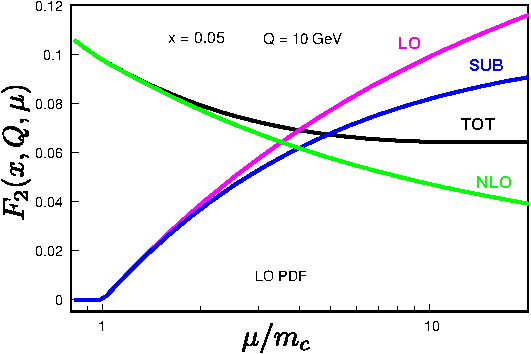
\includegraphics[clip,width=0.45\textwidth]{pics/fred/acot_fig}
\caption{Calculation of $F_{2}^{c}$ vs.\ $\mu$ in the VFNS
  illustrating the cancellation of the LO ($\bar{c}W^{+}\to\bar{s}$)
  and the SUB \hbox{$(g\to
    \bar{c})$}$\otimes$\hbox{$(\bar{c}W^+
    \to \bar{s})$}
  contributions in the region $\mu\sim m_{c}$. The $Q$ scale is fixed
  at $10\,$GeV and the charm PDF is matched at $\mu_{c}=m_{c}$ such
  that $f_{c}(x,\mu=m_{c})=0$. \label{fig:acot}}
\end{figure}

\begin{figure*}
  \centering 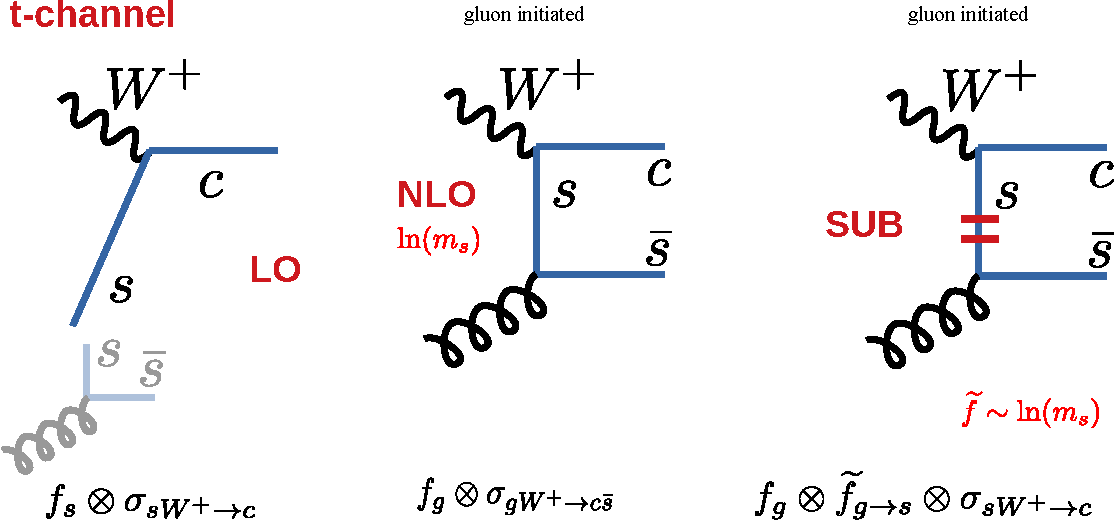
\includegraphics[clip,width=0.8\textwidth]{pics/fred/tchannel}
  \caption{The $t$-channel processes up to ${\cal  O}(\alpha_S^1)$.
Note we sum the combination (NLO$-$SUB) to obtain the complete ${\cal  O}(\alpha_S^1)$ correction;
we find it useful to study these terms separately.
The higher-order quark-initiated contributions are not show, but are included in the calculation. 
\label{fig:tchannel}}
\end{figure*}

\begin{figure*}
  \centering 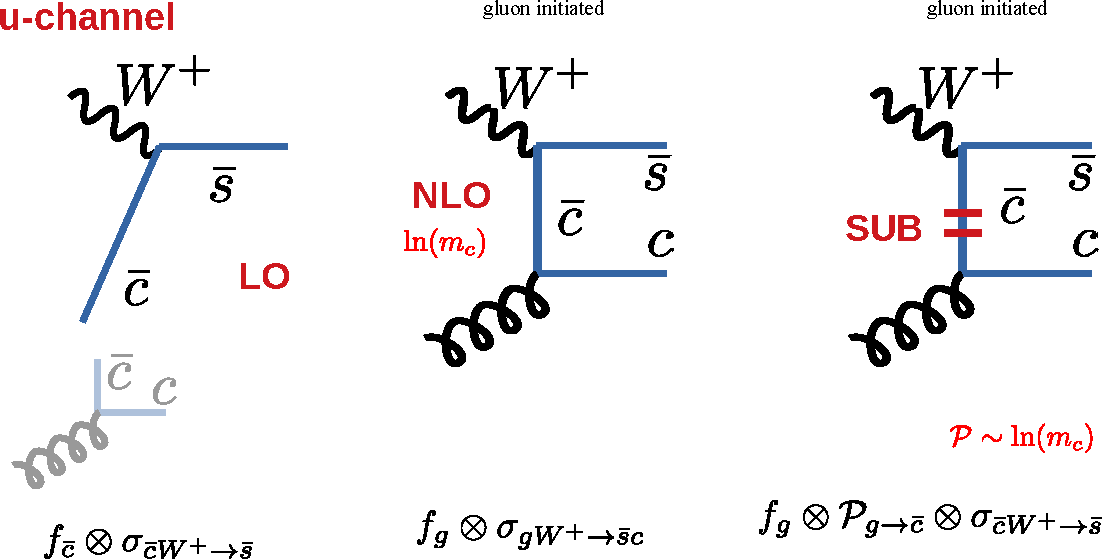
\includegraphics[clip,width=0.8\textwidth]{pics/fred/uchannel}
\caption{The $u$-channel processes  up to ${\cal  O}(\alpha_S^1)$.
Note the NLO  $t$-channel and $u$-channel terms are combined coherently at the amplitude  level. 
The higher-order quark-initiated contributions are not show, but are included in the calculation. 
\label{fig:uchannel}}
\end{figure*}

\xsec{The Multi-Scale Problem:}
%
The CC DIS charm production process involves some interesting issues
that we will explore here in detail. In particular, there are multiple
mass and energy scales which span a wide kinematic range, and it
becomes an intricate puzzle to treat them all properly.

For this current illustration, we will focus on the contribution to
the DIS $F_{2}^{c}$ structure function from the process involving the
strange and charm quark; other quark combinations can be addressed in
a similar manner.
%
The fully inclusive $F_2$ can be studied using the energy and angle of
the outgoing lepton; in contrast, $F_{2}^{c}$ also requires
information about the final hadronic state, and this introduces some
subtleties.
%
In particular, we will show that as we go to higher orders the
$F_{2}^{c}$ structure function must be defined carefully so that: i)
theoretically it is free of divergences and independent of the
renormalization scales when calculated to all orders, 
and ii) experimentally it matches what is
measured by the detector.

%\xsec{Overview:}
%
%\textcolor{blue}{... to be filled in ... (what other detailed are needed???)}

\xsec{The Mass Scales:}
%
What makes this process complex is that we encounter a number of
different mass scales. Furthermore, there is no fixed hierarchy for
the mass scales, and we will need to compute both in the low-$Q$
region, where $Q\lesssim m_{c}$, as well as the high-$Q$ region
$Q\gg m_{c}$.

The $Q$ scale is the invariant mass of the virtual-boson probe
($W^{+}$ in this case), and can be related to the energy and angle of
the lepton; this is a physically measurable kinematic variable.

In contrast, the scale $\mu$ is an unphysical scale which implements
the separation between the PDF and the hard-scattering cross section, 
and the scale at which $\alpha_{s}$ is evaluated;
thus, the physics should be insensitive to a variation of $\mu$. As
our calculations typically involve the dimensionless combination
$\ln(\mu/Q)$, we generally choose $\mu\sim Q$ to avoid large
logarithms.

The strange quark is a ``light'' active parton with an associated PDF
$s(x)$ and mass $m_{s} < \Lambda_{\rm QCD}$. The strange-quark mass is
comparable to or less than other hadronic scales which are neglected;
as such, it serves only as a regulator and plays no physical
role. Effectively, we can take $m_{s}\to 0$ if we choose.
%
We treat the up and down quarks masses $m_{u,d}$ in a similar manner.

The charm quark is a ``heavy'' object; its associated mass
$m_{c}> \Lambda_{\rm QCD}$ does play a physical role and cannot
generally be neglected. There may or may not be a PDF associated with
the charm. In a $n_f=3$ FFNS scheme, we will assume the charm PDF to
be zero.\footnote{It is possible to extend this to incorporate an
  intrinsic-charm PDF.} In a VFNS there is a charm PDF only when the
$\mu$ scale is above the scale where the charm PDF is activated; we
call this the matching scale, $\mu_{c}$.  It is common\footnote{The
  choice of matching scale $\mu_{c}=m_{c}$ is common because at NLO
  the $\overline{\mbox{MS}}$ matching conditions on the PDFs are
  proportional to the DGLAP kernel times $\ln(\mu/m_{c})$. As an
  explicit calculation shows, the constant term vanishes. Therefore,
  by choosing $\mu_{c}=m_{c}$ we have the simple boundary condition
  $f_{c}(x,\mu=m_{c})=0$. At NNLO, the constant term is non-zero and
  this yields $f_{c}(x,\mu=m_{c})\not=0$. See
  Ref.~\cite{Stavreva:2012bs} and references therein.}
%
to set $\mu_{c}=m_{c}$, but this is not required.\footnote{By
  displacing the matching scale to larger values $\mu_{c} > m_{c}$,
  one can have the advantage of avoiding delicate cancellations in the
  region $\mu\sim m_{c}$; this flexibility was explored in
  Refs.~\cite{Bertone:2017ehk,Bertone:2018ids}.}
%
In this study, however, we will adopt this common choice.

Because there are two different quark masses involved ($m_{s}$ and
$m_{c}$) in the CC DIS process, we can examine the mass singularities
of the $t$-channel and $u$-channel separately.
%
This separation is particularly useful to understand how the
individual mass singularities are addressed, and how the FFNS and the
VFNS organize the contributions to the total structure function.

\xsec{The $n_f=3$ FFNS:}
%
To be specific, we will consider CC DIS production of a charm
quark. We first compute this in the $n_f=3$ FFNS where $\{u,d,s\}$ are
light ``active'' partons in the proton, and the charm $c$ is
considered an external ``heavy'' particle. This can be implemented in
the ACOT scheme~\cite{Aivazis:1993pi} for example by using a CWZ
renormalization~\cite{Collins:1978wz} where the light ``active''
partons are renormalized with normal $\overline{\mbox{MS}}$, and the
``heavy'' quarks use a zero-momentum subtraction. In this scheme, the
\textbf{leading-order} (LO) process is \mbox{$sW^{+}\to c$} as
illustrated in Fig.~\ref{fig:acot}. At \textbf{next-to-leading-order}
(NLO), we then include \mbox{$gW^{+}\to c\bar{s}$} which has both
$t$-channel and $u$-channel contributions.\footnote{Note, there are
  also corresponding quark-initiated processes; we will focus on the
  gluon-initiated processes as this is sufficient to illustrate our
  points. Both the gluon- and quark-initiated contributions are
  included in our calculations.}

\xsec{$t$-Channel:}
%
The $t$-channel process has an intermediate $s$-quark exchanged, and
if we use the strange quark mass $m_{s}$ to regulate the
singularities, this will yield a contribution proportional to
$\ln(Q/m_{s})$. This mass singularity arises from the region of phase
space where the exchanged $s$-quark becomes collinear and close to the
mass shell; that is, when the phase space of the
\mbox{$gW^{+}\to c\bar{s}$} process begins to overlap with that of the
\mbox{$sW^{+}\to c$} process. This ``double counting'' is resolved by
a \textbf{subtraction} (SUB) counter-term
%(which is formally part of the NLO contribution)
given by:
\[
(SUB)\sim f_{g}\otimes\widetilde{f}_{g\to s}\otimes\sigma_{sW^{+}\to
  c}\,.
\]
Here, $\widetilde{f}_{g\to s}$ is the perturbative splitting of the
gluon into an $s\bar{s}$ pair; the leading term is proportional
to:\footnote{The scale of the SUB term is $\mu$ as the relevant scale
  here is the renormalization scale of the PDF:
  $f(x,\mu)\otimes\hat{\sigma}(x,Q,\mu)$.}
\[
\widetilde{f}_{g\to s}(x,\mu)\sim\frac{\alpha_{S}(\mu)}{2\pi}P_{g\to
  s}^{(1)}(x)\:\ln\left(\frac{\mu^{2}}{m_{s}^{2}}\right)+\text{{\cal
    O}}(\alpha_{s}^{2})
\]
where $P_{g\to s}^{(1)}(x)$ is the $\mathcal{O}(\alpha_{s})$ DGLAP
splitting kernel for \hbox{$g\to s$}.

The complete contribution to the structure function is given by:
\[
F_{2}^{c}\sim TOT=LO+(NLO-SUB)
\]
The complete ${\cal O}(\alpha_{s})$ contribution is the combination
$(NLO-SUB)$; our separation into $NLO$ and $SUB$ is simply to
illustrate the interplay of these components. Both the NLO and SUB
terms have $\ln(m_{s})$ divergences, but these precisely cancel and
yield a well defined result even as we take the $m_{s}\to 0$
limit.\footnote{In fact, we could have taken $m_{s}=0$ initially and
  used dimensional regularization to compute the contributions.}

\xsec{$u$-Channel:}
%
We next examine the $u$-channel NLO contribution to the
\mbox{$gW^{+}\to c\bar{s}$} process. This has an intermediate
$c$-quark exchanged and is proportional to $\ln(Q/m_{c})$. In the FFNS
where the charm is a ``heavy'' non-parton, there is no counter-term
for this graph, and the resulting observables will retain the
$\ln(Q/m_{c})$ dependence. In principle, this means that when we go to
large $Q$ scales, these terms will begin to degrade the convergence of
the perturbative series. In practice, while this degradation only
grows logarithmically, at large scales (such as at the LHC energies)
we do find it convenient to treat the charm on an equal-footing as the
${u,d,s}$ partons.

\xsec{The VFNS:}
%
We now turn to the VFNS scheme where we include the charm quark as an
``active'' parton and compute its associated PDF.

In this case, there is a $u$-channel counter-term (SUB) given by
$f_{g}\otimes\widetilde{f}_{g\to\bar{c}}\otimes\sigma_{\bar{c}W^{+}\to\bar{s}}$
which is proportional to $\ln(\mu/m_{c})$. The NLO $u$-channel
contribution will have a $\ln(Q/m_{c})$ factor, so the combination
$(NLO-SUB)$ is also free of mass singularities.\footnote{Specifically,
  the combination $(NLO-SUB)$ is free of mass singularities and finite
  in the limit $m_{c}\to0$. Note that the VFNS fully retains the charm
  quark mass $m_{c}$ and (in contrast to some claims in the
  literature) the factorization holds up to
  ${\cal O}(\Lambda^{2}/Q^{2})$ corrections; all terms of order
  $(m_{c}^{2}/Q^{2})$ are fully included~\cite{Collins:1998rz}.}

What is less obvious is that we must also include the LO process
\mbox{$\bar{c}W^{+}\to\bar{s}$}. There are two ways we can understand
why this is necessary.

\xsec{Explanation \#1: Matching of LO and SUB:}
%
Recall that in the $t$-channel case, the subtraction term SUB removed
the double counting between the LO \mbox{$sW^{+}\to c$} and NLO
\mbox{$gW^{+}\to c\bar{s}$} subprocesses.

The $u$-channel case is analogous in that this subtraction term
removes the double counting between the LO
\mbox{$\bar{c}W^{+}\to\bar{s}$} and NLO \mbox{$gW^{+}\to c\bar{s}$}
subprocesses; both contributions are required to ensure the resulting
cross section is insensitive to the scale $\mu$.

This is apparent in Fig.~\ref{fig:acot} where we plot the individual
terms versus $\mu$ for fixed values of \xbj and $Q$. In the region
$\mu\sim m_{c}$, the charm PDF $f_{c}(x,\mu)$ (and hence, the LO
contribution) rises very quickly as the DGLAP evolution is driven by
the very large gluon distribution via $g\to c\bar{c}$ splitting, and
combined with a large $\alpha_{s}(\mu)$. The SUB subtraction also
rises quickly as this is driven by the logarithmic term
$\ln(\mu^{2}/m_{c}^{2})$. The difference \mbox{$(LO-SUB)$} is the
physical contribution to the total \mbox{$[TOT=LO+NLO-SUB]$}, and it
is this combination which is smooth across the ``turn on'' of the
charm PDF at the matching scale $\mu_{c}=m_{c}$.  We now see that if
we neglect the LO \mbox{($\bar{c}W^{+}\to\bar{s}$)} contribution, we
lose the cancellation between LO and SUB in the region
$\mu\sim m_{c}$, and our structure function (or cross section) would
have an anomalous shift at the arbitrarily location $(\mu_{c})$ where
we turn on the charm PDF.

As we vary the unphysical scale $\mu$, we are simply shifting
contributions between the separate \mbox{$\{LO,NLO,SUB\}$} terms which
individually exhibit a large $\mu$-dependence. However, the total
combination $(TOT)$, which represents the physical observable, is
relatively insensitive to $\mu$ (up to higher orders), and this
property is evident in Fig.~\ref{fig:acot}.

\xsec{Explanation \#2: Removing ``Double Counting:''}
%
A second way to understand why we require the LO process
\mbox{$\bar{c}W^{+}\to\bar{s}$} is to consider the regions of phase
space covered by each of the subprocesses. The singularity of the
$u$-channel NLO \mbox{$gW^{+}\to c\bar{s}$} processes arises from the
phase-space region when the intermediate $\bar{c}$-quark becomes
collinear and close to the mass shell.\footnote{For example, the
  $c$-quark is off-shell by the order of its mass $m_{c}$; this is
  independent of the scale $Q$ and \textit{does not} assume any
  $Q\gg m_{c}$ limit.} This is precisely the phase-space region of the
LO process \mbox{$\bar{c}W^{+}\to\bar{s}$} where the partonic
$\bar{c}$-quark is collinear to the hadron. The SUB term then removes
the ``double counting'' between the LO and NLO contributions; hence,
all three contributions \mbox{$\{LO,NLO,SUB\}$} are necessary to cover
the full phase space.

This is also apparent if we consider the transverse momentum $(p_{T})$
of the final-state charm in the Breit frame. For the LO
\mbox{$\bar{c}W^{+}\to\bar{s}$} process in the Breit frame, the
incoming $W^{+}$ and $\bar{c}$ are collinear, and the produced
$\bar{s}$ must have zero $p_{T}$ in this frame.

For the NLO $gW^{+}\to c\bar{s}$ process, we integrate over the
complete phase space for the exchanged $\bar{c}$ quark, and this will
include the region where the $\bar{c}$-quark is emitted nearly
collinear to the gluon and nearly on-shell; in this region the
$\bar{c}$-quark will have $p_{T}\sim 0$ and we encounter a singularity
from the internal $\bar{c}$-quark propagator. The $p_{T}\sim 0$ region
is precisely that subtracted by the SUB counter
term\footnote{Specifically, the incoming $W^{+}$ and $g$ are
  collinear and the gluon then emits a collinear $c\bar{c}$ pair so
  the final $\bar{s}$ has zero $p_{T}$.} and this ensure that the
combination $(NLO-SUB)$ is free of divergences.

\xsec{Recap:}
%
To recap, i) the combination of the LO and SUB terms ensure a minimal
$\mu$ variation at low $\mu$, and ii) the combination of SUB and NLO
ensures that the mass singularities are canceled at high $\mu$.

This interplay of the terms illustrates some of the intricacies of
QCD, especially since this exchange is across different orders of
$\alpha_{s}$.

Furthermore, note that in the $u$-channel for both the LO and SUB
contributions, the charm quark is collinear to the incoming hadron,
and thus exits in the hadron remnants. While this may be
experimentally difficult to observe, because we are asking for a
\textit{``fully inclusive''} $F_{2}^{c}$, these contributions cannot
be simply ignored. We will discuss this further in the following
section.

\xsec{Defining $F_{2}^{c}$:}
%
The LO $u$-channel \mbox{$\bar{c}W^{+}\to\bar{s}$} process foreshadows
difficulties that we encounter if we try and extend the concept of a
``fully inclusive'' $F_{2}^{c}$ to higher orders. We note that in
Ref.~\cite{Collins:1998rz} Collins extended the proof of factorization
to include heavy quarks such as charm and bottom for an inclusive
structure function $F_{2}$; there is no corresponding proof for an
\textit{``fully inclusive''} $F_{2}^{c}$.
%
Whereas $F_2$ only requires measurement of the outgoing lepton energy
and angle, $F_2^c$ also requires information on the final state.  At
the parton level, this introduces complications including when the
charm is in the hadronic remnants and brings in both fragmentation and
fracture functions.

To characterize the theoretical issues involved in constructing
$F_{2}^{c}$, we can imagine starting from the (well-defined) inclusive
$F_{2}$, and then dividing the contributions into two sets: one for
$F_{2}^{c}$ for the ``heavy'' charm quark, and the rest into
$F_{2}^{u,d,s}$ for the ``light'' quarks. We will show that this
theoretical procedure encounters ambiguities.

The LO $u$-channel $\bar{c}W^{+}\to\bar{s}$ process does not have any
``apparent'' charm quark in the final state, but this contribution is
essential to balance with the SUB process
\mbox{$f_{g}\otimes\widetilde{f}_{g\to\bar{c}}\otimes\sigma_{\bar{c}W^{+}\to\bar{s}}$.}
Note that for the SUB process the charm quark arises from a gluon
splitting into a collinear $c\bar{c}$ pair which is then part of the
hadron remnants. For the LO process, presumably our $\bar{c}$ quark
also came from a gluon splitting into a collinear $c\bar{c}$
pair. Thus, our $F_{2}^{c}$ must include those cases where the charm
is contained in the hadron remnants.

This issues touches on the fact that, because the charm parton
ultimately fragments into a charmed hadron (typically a $D$ meson), we
must introduce a set of fragmentation functions (FFs) which are
scale-dependent and will factorize final-state singularities in a
similar manner as the PDFs factor the initial-state
singularities.\footnote{For the NLO quark-initiated contributions (not
  shown) we will have final state singularities from processes such as
  $c\to cg$ which will be factorized into the FFs.} Note that we also
may allow for the possibility that a gluon or a light quark can
produce a charmed hadron pair.

\xsec{The Bubble  Diagram:}
%
\begin{figure}[t]
\centering 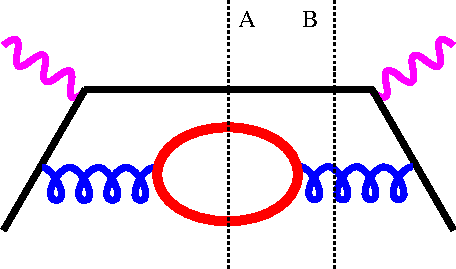
\includegraphics[width=0.45\textwidth]{pics/fred/feyngraph}
\caption{A higher order Feynman graph illustrating the complications
  in defining a ``fully inclusive'' $F_{2}^{charm}$.  A light quark
  ($q$) scatters from a vector boson ($V$) with a $c\bar{c}$ in the
  internal loop.  If we cut the amplitude at ``A'' we have charm in
  the final state and this must be included in $F_{2}^{charm}$.  If we
  cut the amplitude with cut ``B'' there is no charm in the final
  state.  Additionally, since this diagram contributes to the beta
  function, this highlights the complications of using an $\alpha_{S}$
  and hard scattering $\hat{\sigma}$ with differing $N_{\rm
    eff}$. \label{fig:bubble}}
\end{figure}

Some of the theoretical intricacies of defining a \textit{``fully
  inclusive''} $F_{2}^{c}$ are illustrated in Fig.~\ref{fig:bubble}
which shows a higher-order DIS process with a quark-antiquark loop.

Let us compute this diagram in the $n_f=3$ FFNS where the internal
loop is a massive $c\bar{c}$-pair and the external quark is a light
quark \mbox{$\{u,d,s\}$}.  If the final state is represented by Cut-A,
then we have charm quarks in the final state, and this should be
included in $F_{2}^{c}$.

However, if we instead use Cut-B as a final state, there is no charm
in the final state, so this should not be included in $F_{2}^{c}$.
[More precisely, when we renormalize the charm loop with zero-momentum
subtraction, this contribution effectively decouples.] Thus, the
contribution from Cut-A will be included in $F_{2}^{c}$, but the
contribution from Cut-B will not.

This diagram generates additional complications in that multiple quark
flavors are involved. For example, the bubble diagram involves quarks
of both $q=\{u,d,s\}$ and $c$ flavors, so this contribution cannot be
uniquely assigned to $F_{2}^{q}$ or $F_{2}^{c}$. We can introduce
theoretical definitions to make the choice, but then we have to be
careful about double-counting contributions and introducing
uncancelled singularities.
%
For example, the bubble diagram of Fig.~\ref{fig:bubble} is
encountered in the $F_{2}^{c}$ heavy-quark calculations of
Refs.~\cite{Chuvakin:1999nx,Chuvakin:2000jm}; here, an additional
scale $\Delta$ is introduced to subdivide the contributions.

\xsec{The running $\alpha_{s}$ in the FFNS:}
%
The bubble diagram of Fig.~\ref{fig:bubble} also highlights the
difficulty of using a $n_f=3$ FFNS with a VFNS running of
$\alpha_{s}$. In a $n_f=3$ FFNS, internal $c\bar{c}$ loops decouple
from the theory and are not included in the calculation;\footnote{More
  precisely, the heavy quarks are renormalized with zero-momentum
  subtraction and their contributions decouple; this is why we can
  neglect loops from the the top quark and any other heavy particle.
} however, the $\beta$-function with $n_f=4$ requires precisely these
$c\bar{c}$ loop contributions. Note that this deficiency can be
patched order-by-order by expanding the $\beta$-function and inserting
the required terms at each
order~\cite{Napoletano:2014thesis,Bierenbaum:2009zt,Cascioli:2013era}.
Once again, we cannot unambiguously divide the inclusive $F_{2}$ into
separate ``light'' and ``heavy'' quantities.

\xsec{Extensions to bottom and top:}
%
While we have used the charm quark to illustrate these features, the
same properties can, in principle, be applied to both the bottom and
top quark.\footnote{Additionally, Collins definitively addressed the
  case of multiple heavy quarks which can allow for both charm and
  bottom in a unified framework; in contrast to some incorrect claims
  in the literature, there is no difficulty in including multiple
  heavy quarks. (\textit{cfr.} Ref.~\cite{Collins:1998rz}, Sec.~IX.)}
For the case of the bottom quark, the larger mass $m_{b}$ yields a
smaller $\alpha_{s}(\mu)$ for $\mu\sim m_{b}$ and the evolution of
$f_{b}(x,\mu)$ is thus reduced. Nevertheless, for large scale
processes (such as at the LHC) we often find it convenient to make use
of $f_{b}(x,\mu)$ and treat the bottom on an equal footing as the
other light quarks.
%
For the case of the top quark, the very large mass $m_{t}$ yields a
much smaller $\alpha_{s}(\mu)$ for $\mu\sim m_{t}$ and the evolution
of $f_{t}(x,\mu)$ is comparatively reduced.

\subsection*{Summary}

To properly define an $F_{2}^{c}$ at higher orders, we encounter the
theoretical issues discussed above: as the charm quark fragments into
a charmed meson, we must be careful to ensure that the theoretical
quantity matches what is actually measured experimentally.
%
This is more complex than simply asking for the portion of $F_{2}$
which has charm in the final state, and is an issue for both the FFNS
and VFNS as we move to higher orders.
%
We can perform the computation in the FFNS but in the large energy
limit we encounter $\ln(Q^{2}/m_{c}^{2})$ divergences and this, in
part, contributes to the observed differences at large $Q$.

The VFNS includes the charm quark as an active parton for $\mu$ scales
above a matching scale $\mu_{c}$. For large $Q$ scales, the mass
singularities of NLO and SUB will cancel to yield a result free of
divergences. For scales $\mu\sim m_{c}$, cancellation between the LO
and SUB contributions ensures minimal $\mu$ dependence; however, as
this can be delicate to implement numerically, we have the option of
displacing the matching scale $\mu_{c}$ to a larger scale where the
cancellation is more stable~\cite{Bertone:2017ehk,Bertone:2018ids}.


%\subsection*{Acknowledgements}
%Thanks to:
%John Collins, Ted Rogers, George Sterman, Ingo Schienbein, Aleksander Kusina

%\bibliographystyle{unsrt}
%\bibliography{fred}

%\end{document}
